\subsection{Analyisis}

As seen in Figure \ref{5_ctv-optimal-ctv}, the \algorithmBalanced{}{} algorithm in the simple system optimises the system utility by $XXX\%$, from $XXX\%$ in the first episode through to $XXX\%$ by episode $500$.
\begin{figure}[ht]
	\centering
	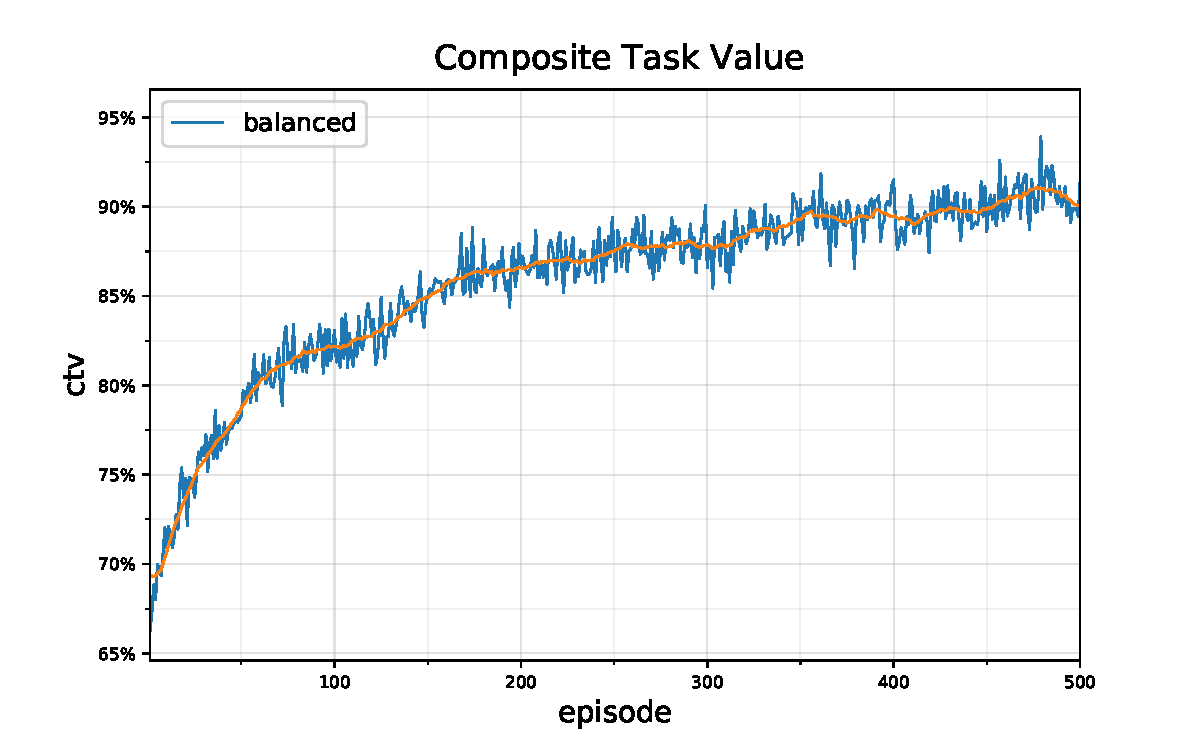
\includegraphics[width=0.8\linewidth]{5_ctv-optimal-ctv}
	\captionsetup{labelfont=bf,singlelinecheck=on}
	\caption{System utility compared to the theoretical maximum for the \simulationSimple{}{} system. The algorithms work to increase this value, which impacts the task values, energy consumption, and distribution depending on the weighting given to those various components}
	\label{fig:5_ctv-optimal-ctv}
\end{figure}
In Figures \ref{fig:5_ctv-statistics-energy-available}, \ref{fig:5_ctv-quality}, we see the impact of the CTV optimisation on task values and available system energy. The average quality of the measurement tasks as compared to the optimal quality available in the sytem given the agents distance from the respective tasks' demand points. Over the systems' lifetime this is increased from $XXX\%$ to $XXX\%$. Similarly as the algorithm improves the routing for task allocation, the energy consumption of the system is reduced, the available energy going from  $XXX\%$ to $XXX\%$. These results demonstrate the the algorithm meets the described problems requirements of allocating tasks to increase their value, while optimising the energy usage as it does so.
 
\todo[inline]{Need a quality fdiagram here}
\begin{figure}[ht]
	\centering
	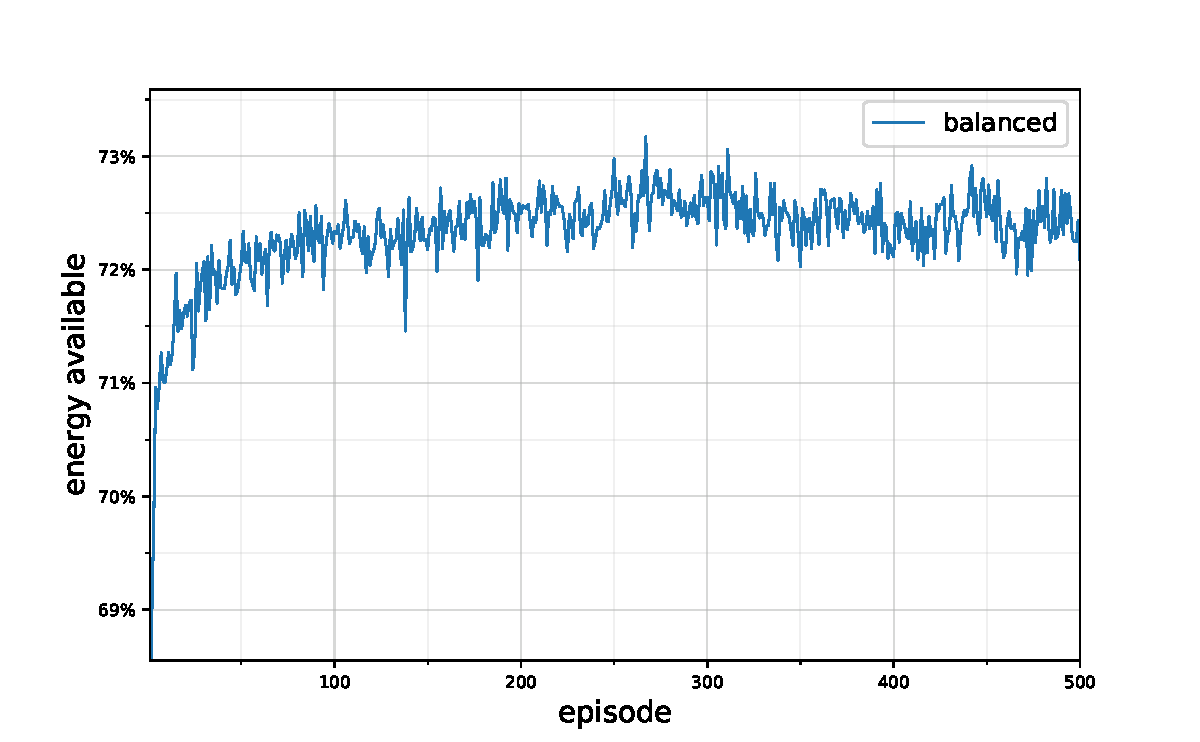
\includegraphics[width=0.8\linewidth]{5_ctv-statistics-energy-available}
	\captionsetup{labelfont=bf,singlelinecheck=on}
	\caption{Energy available in the \simulationSimple{}{} system as percentage of the maximum possible. Higher values show a more efficient use of agents to complete tasks, but may not give the best task values overall}
	\label{fig:5_ctv-statistics-energy-available}
\end{figure}
\begin{figure}[ht]
	\centering
	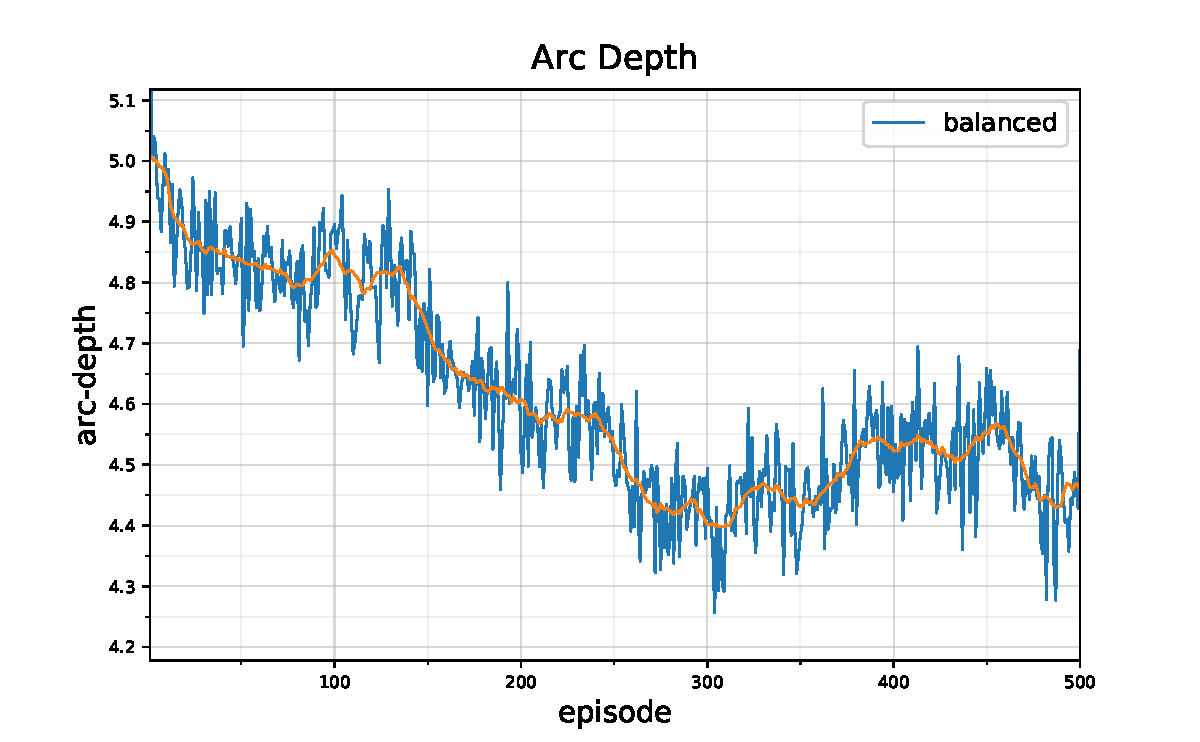
\includegraphics[width=0.8\linewidth]{5_ctv-arc-depth}
	\captionsetup{labelfont=bf,singlelinecheck=on}
	\caption{The average depth of arcs in the \simulationSimple{}{} system. Longer arcs allow sink agents to reach sensing agents that are closer to the task demand point, at the cost of greater energy usage}
	\label{fig:5_ctv-arc-depth}
\end{figure}
\begin{figure}[ht]
	\centering
	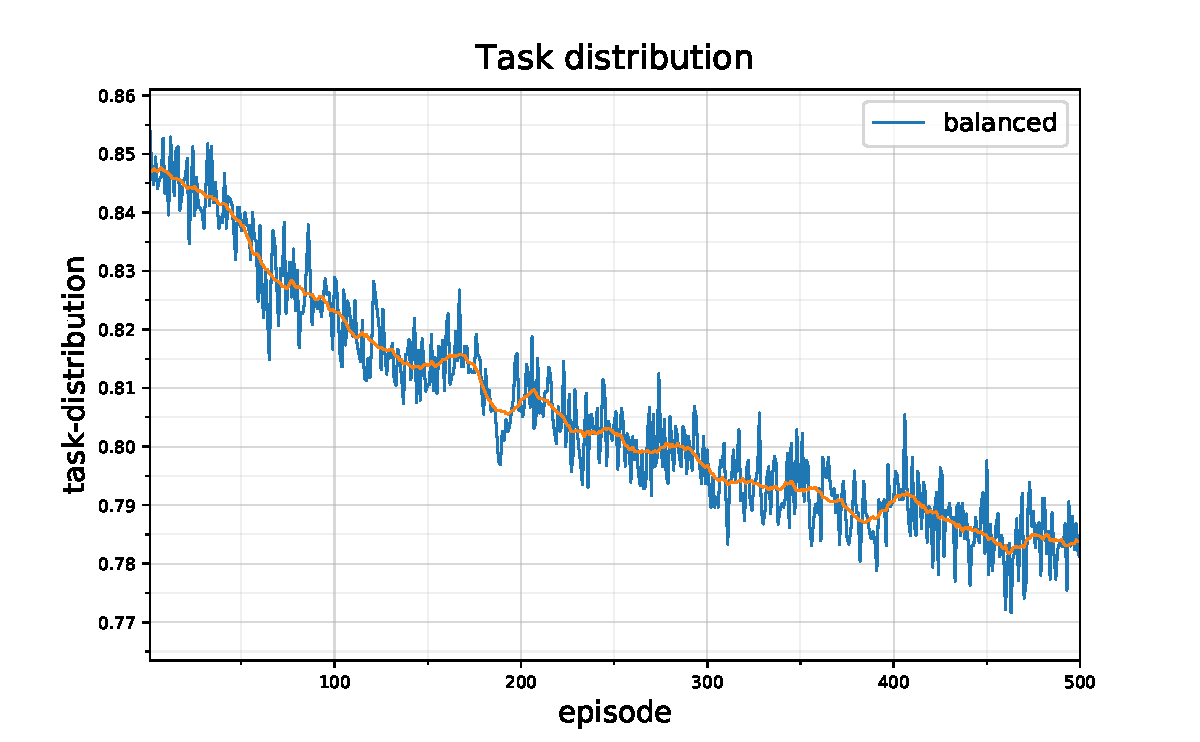
\includegraphics[width=0.8\linewidth]{5_ctv-task-distribution}
	\captionsetup{labelfont=bf,singlelinecheck=on}
	\caption{The task distribution in the system. Higher values spread energy usage across the system better, increasing the systems' lifetime}
	\label{fig:5_ctv-task-distribution}
\end{figure}

We see the ability of the algorithm to weight its optimisation between task quality, energy availability, and distribution given varying values for the $\alpha, \beta, \gamma$ parameters in Figures \ref{fig:5.19_ctv-quality-energy} and  \ref{XXX}. Figure \ref{fig:5.19_ctv-quality-energy} shows the task quality/energy availability of the system. As values range higher, this means that quality is being preferentially optimised for over energy availability. As expected, the \algorithmQuality{}{} algorithm, with its high $\gamma$ value increases this fraction from $XXX\%$ to $XXX\%$ over the system lifetme, whereas the \algorithmEnergy{}{} algorithm moves from only $XXX\%$ to $XXX\%$, a comparatively small increase. As seen, system utility, the sum of CTVs, and energy availability are optimised in both these systems, however it is the relative increase in the task quality and energy availability that is different, showing that the CTV used within the algorithm optimises across these multiple objectives flexibly. 



\begin{figure}
	\centering
	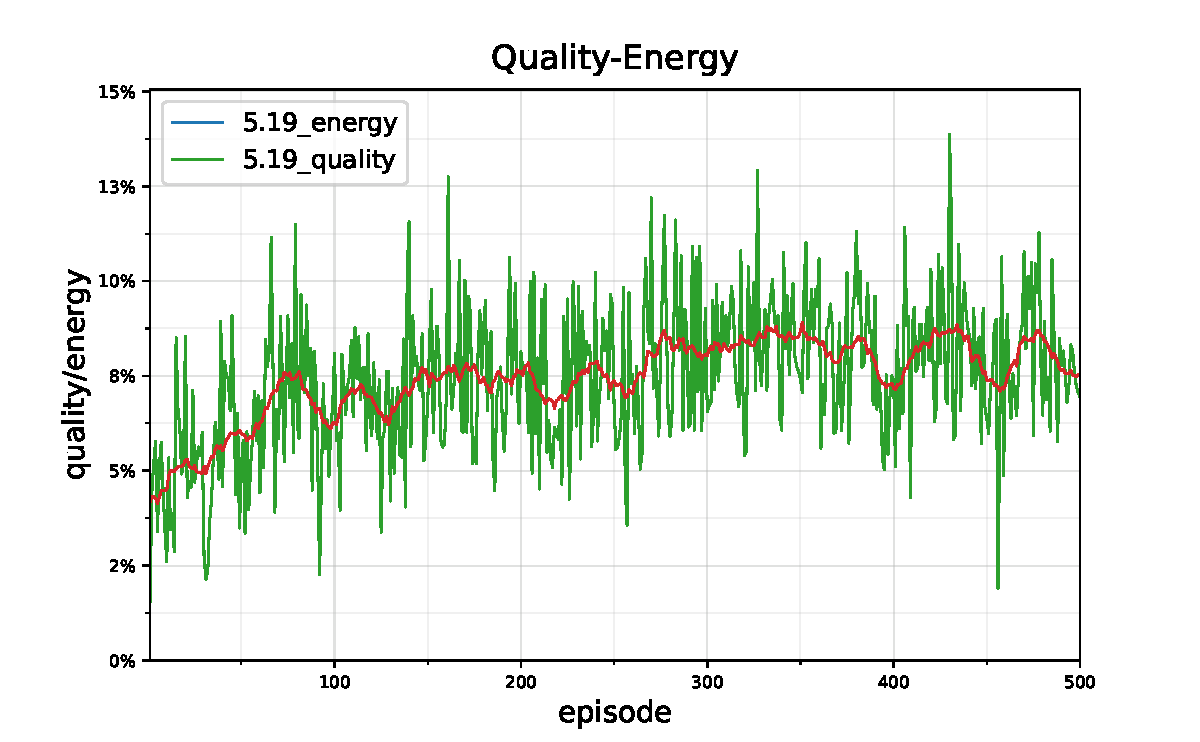
\includegraphics[width=0.7\linewidth]{5.19a_ctv-quality-energy-baseline-comparison}
	\caption{}
	\label{fig:5}
\end{figure}
\begin{figure}
	\centering
	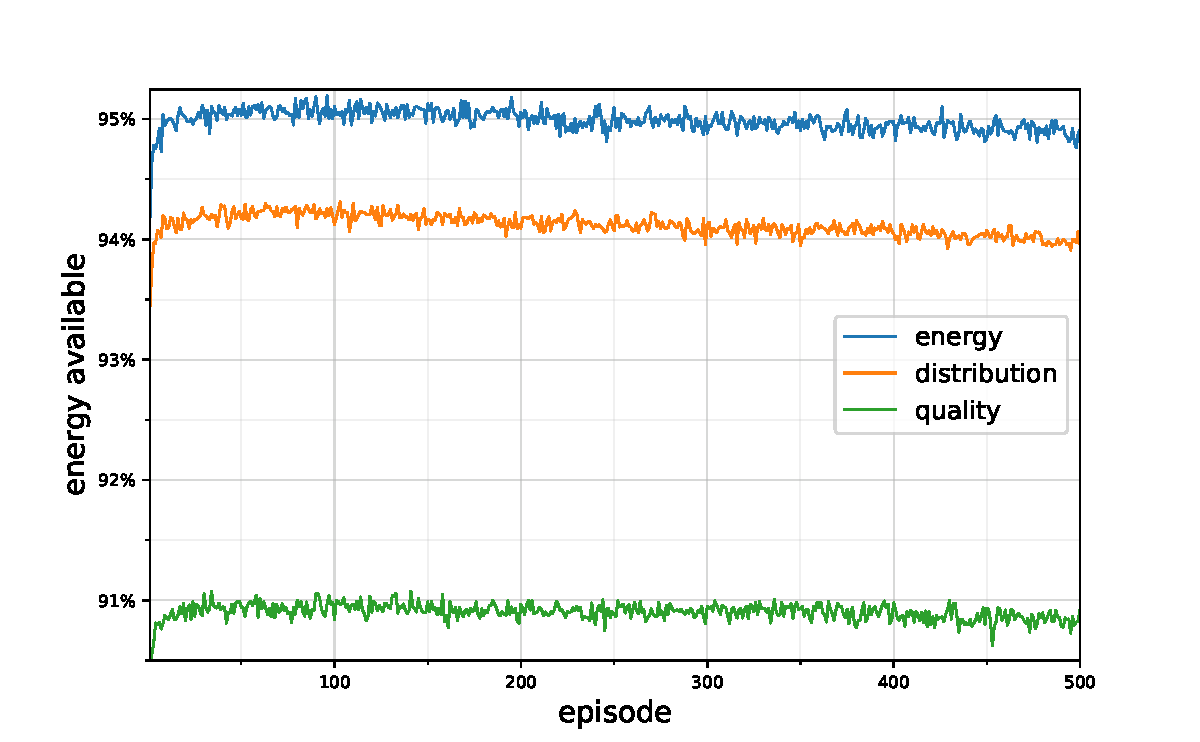
\includegraphics[width=0.7\linewidth]{5.19_ctv-statistics-energy-available-comparison}
	\caption{}
	\label{fig:5}
\end{figure}
\begin{figure}
	\centering
	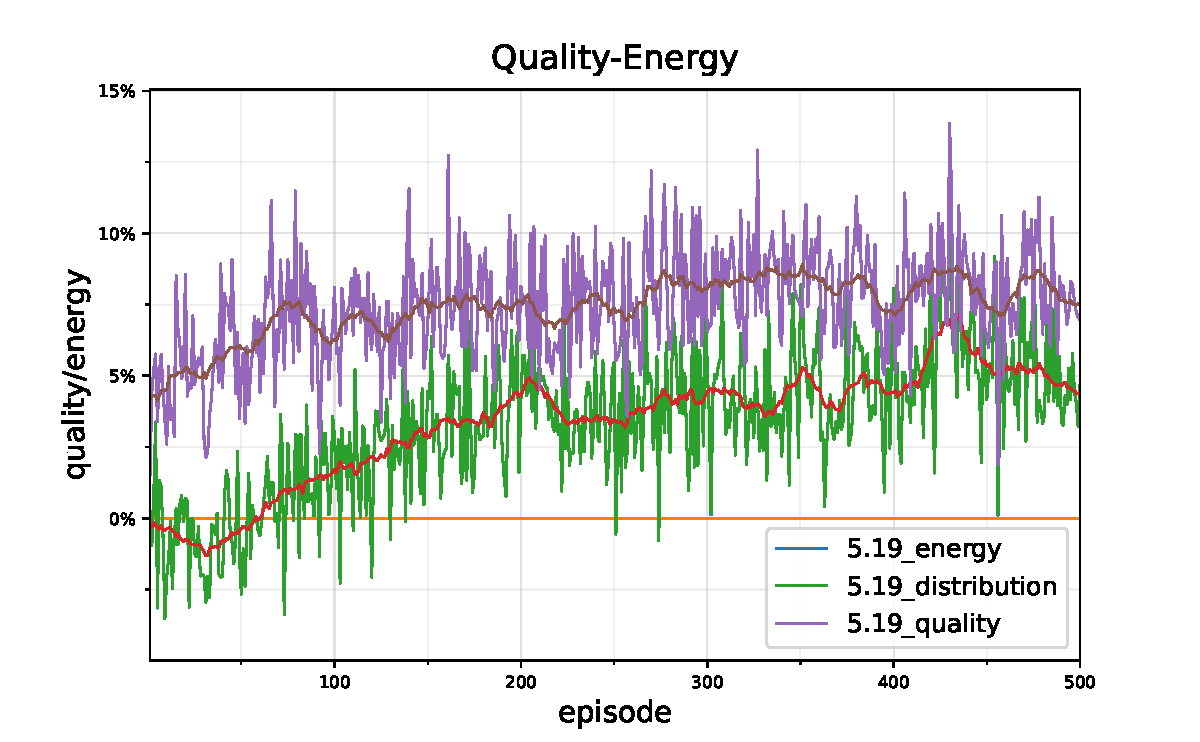
\includegraphics[width=0.7\linewidth]{5.19_ctv-quality-energy-baseline-comparison}
	\caption{}
	\label{fig:5}
\end{figure}
\begin{figure}
	\centering
	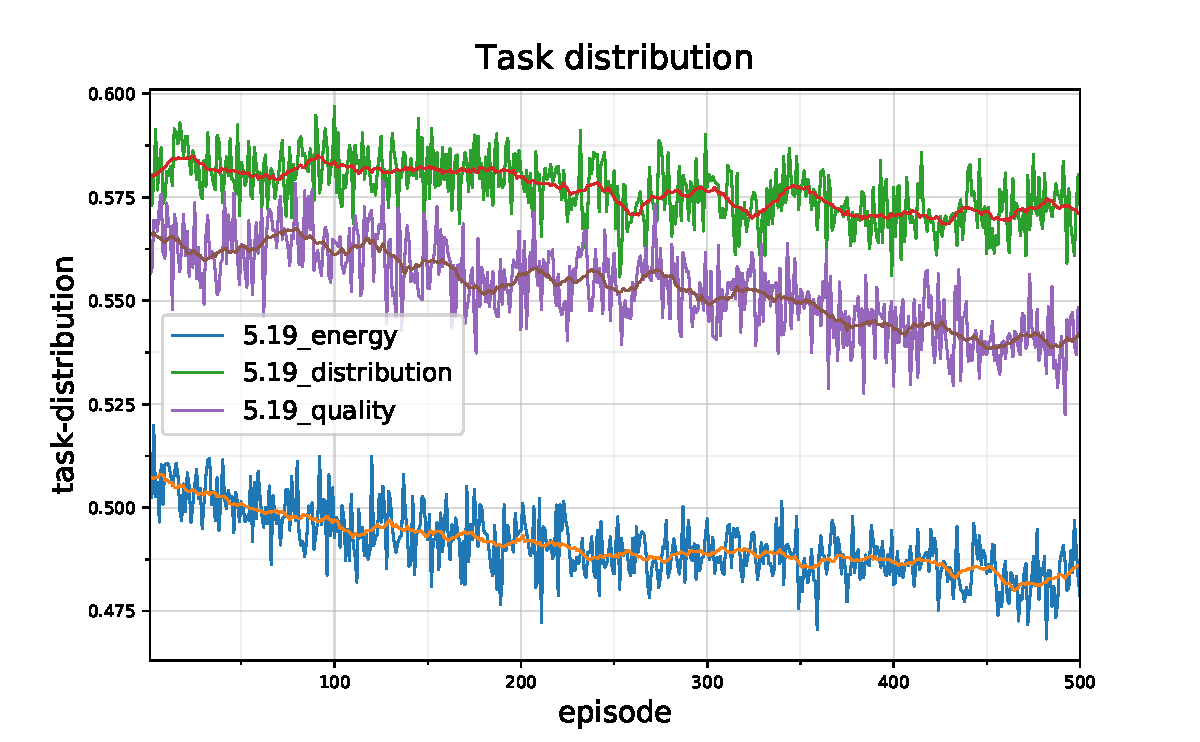
\includegraphics[width=0.7\linewidth]{5.19_ctv-task-distribution-comparison}
	\caption{}
	\label{fig:5}
\end{figure}
\begin{figure}
	\centering
	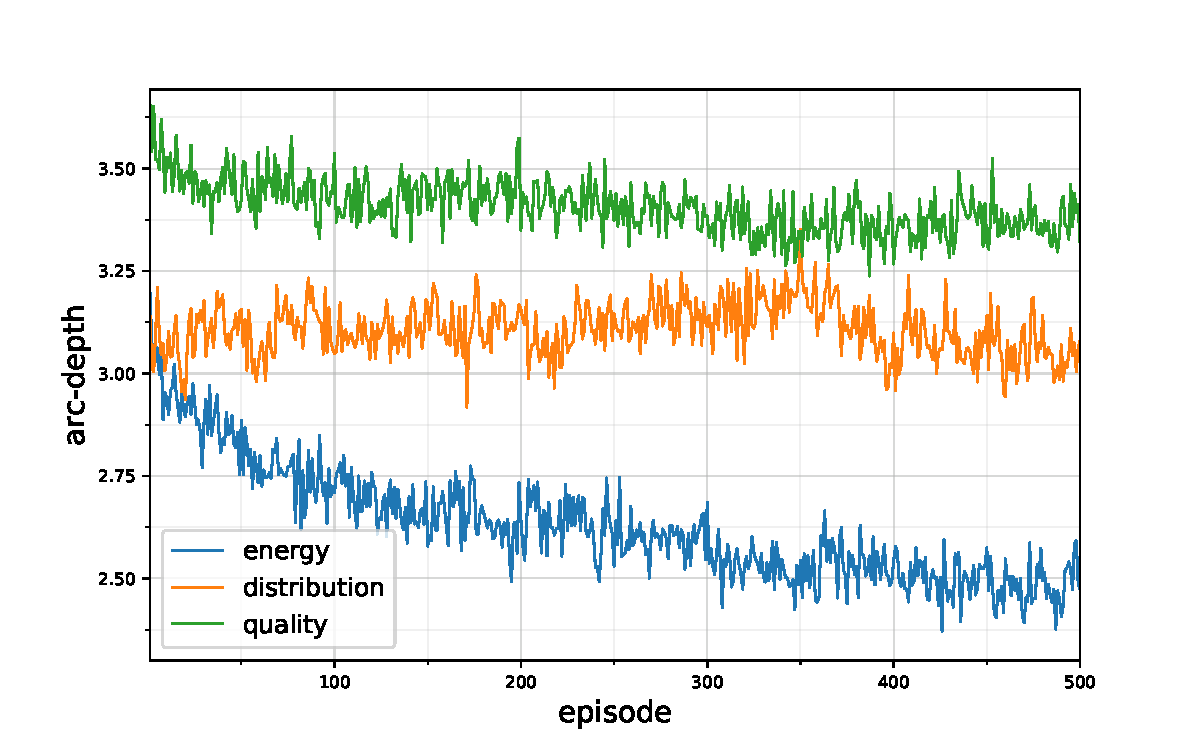
\includegraphics[width=0.7\linewidth]{5.19_ctv-arc-depth-comparison}
	\caption{}
	\label{fig:5}
\end{figure}

\begin{figure}
	\centering
	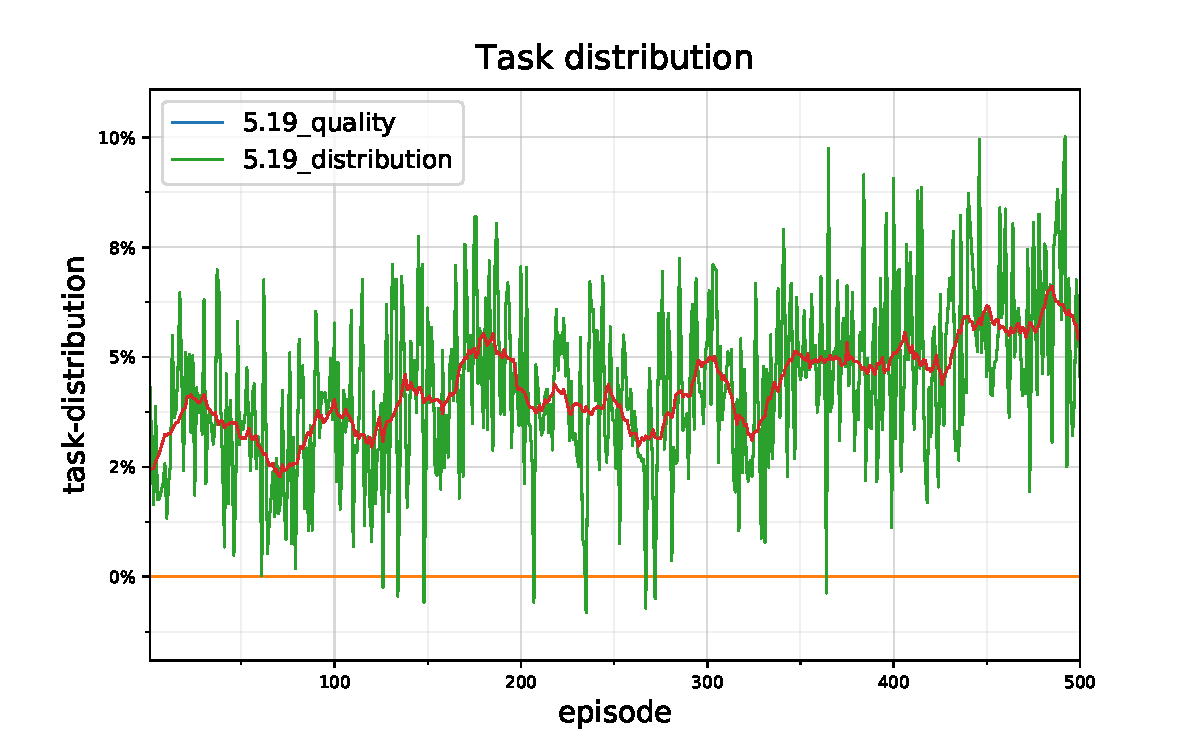
\includegraphics[width=0.7\linewidth]{5.19c_ctv-task-distribution-baseline-comparison}
	\caption{}
	\label{fig:5}
\end{figure}

